\documentclass{standalone}

\begin{document}

\subsection[Yolo]{Yolo architecture}\label{obj_detection:yolo}

\begin{center}
\begin{figure}[htbp]
\centering
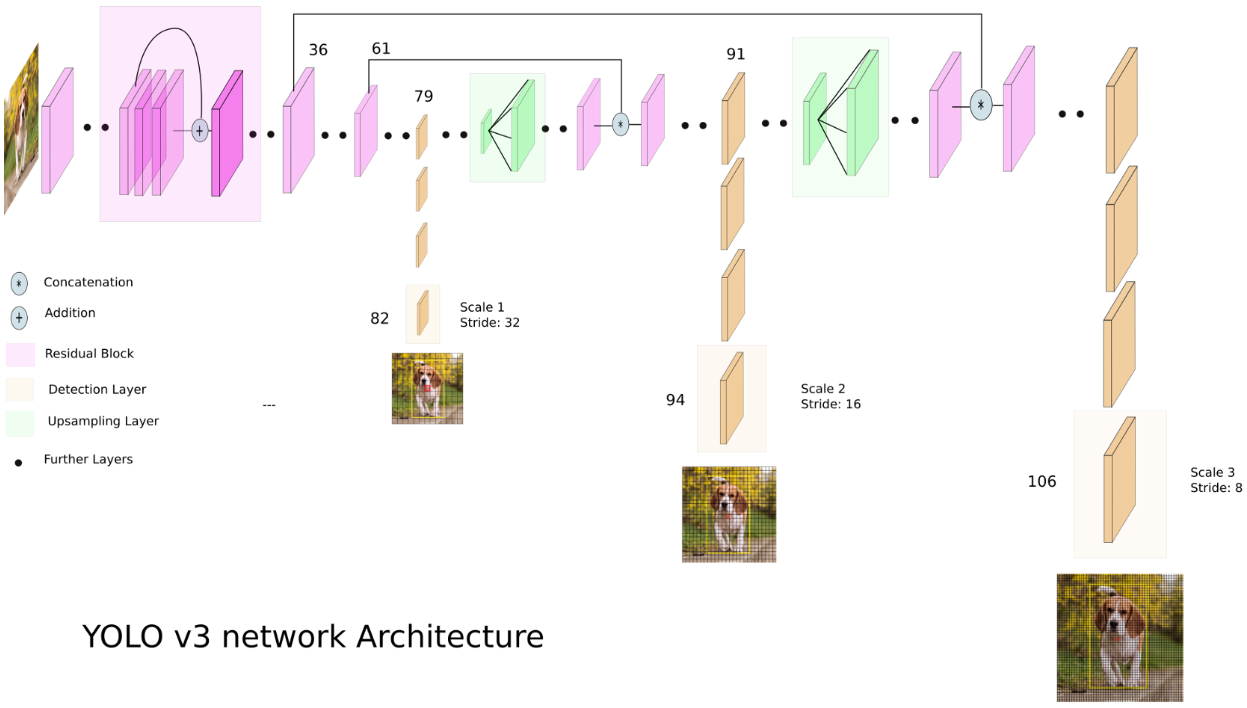
\includegraphics[width=0.85\textwidth]{yolonet.png}
\caption{Yolo Neural Network scheme.
}
\label{fig:yolo}
\end{figure}
\end{center}

YOLO Neural Network architecture was firstly published in the 2015, but from the first version many improvements have been performed and now we have the third version of it.
We do not want to recall the history of this model, so we will discuss only about the YOLOv3 model (for sake of simplicity we will call it just YOLO).

YOLO is a deep Neural Network model with more than 100 layers and more than 62 million of parameters.
The first versions of YOLO was based on a Darknet-19 architecture ($19$-layers Neural Network followed by $11$ more layers for object detection).
In the last release of YOLO the first part of the network structure is used for the feature map extraction and it is essentially a modified version of the Darknet-53 model, i.e the updated version of the previous model, with more layers and parameters.
These improvements increase classification performances but it throwbacks a reduction in computational performances\footnote{
  For the record, the older YOLO version are faster than the last release but less accurate.
}.
These improvements could be done also thank to the introduction of multiple residual blocks which, as discussed in the previous sections (ref. \ref{NN:shortcut}), allow to increase the deep of the model without losing performances.

YOLO performs object detection using a multi-scale approach: three different scales are taken into account during the training section to improve classification performances.
The network structure can be broadly summarized as a simple CNN and its output is generated by applying a series of three different detection $1\times1$ kernels on the feature map.
Moreover, this detection is performed in three different places into network, i.e three YOLO detection layers are distributed along the network structure.
The detection kernel shape is $1\times1\times(B\times(5 + C))$, where $B$ is the number of bounding boxes which a cell in the feature map can predict and $C$ is the number of classes.
The fixed number (\quotes{$5$}) is given by $4$ bounding boxes attributes plus $1$ object confidence coefficient (the so-called \emph{objectness} into the code).
In our applications we have used the COCO dataset (see next sections, \ref{obj_detection:coco}) and thus we have fixed the value of $B$ and $C$ to $3$ and $80$, respectively (thus the kernel size is equal to $1\times1\times255$).
We would stress that the three scale detections are equivalent to three levels of down-sampling of the original image (or better the feature map), respectively equal to $32$, $16$ and $8$.

The input image is down-sampled using the first $81$ layer and only the $82$nd layer performs the first detection\footnote{
  Considering an input image of size $416\times416$ the resulting feature map would be of size $13\times13$.
}.
Then the feature map produced by the $79$th layer is subjected to few convolutional layers before being $2$x up-sampled to a $26\times26$.
The up-sampling is performed by a previously discussed Upsample function/layer (ref. \ref{SR:downsampling}).
The feature map is then concatenated with the one produced by the $61$st layer and it is processed by a second series of convolutions up to the $94$th layer performs the second detection.
A third (similar) procedure is performed again up to the end of the architecture ($106$th layer), where the final $52\times52\times255$ feature map is produced as output.
The first detection layer is responsible for detecting larger objects, while the second two analyze smaller regions: a comparative analysis of these three different scale results improves the detection performance and it help to filter false positive detections.

The introduction of three different detection layers improves the detection of small objects in comparison to the previous versions, but it remains a crucial limit of the model.
Moreover, the up-sampling layers connected with the previous layers (shortcut) help to preserve the fine grained features and thus the identification of small objects into the image.

The model uses a total of $9$ anchor boxes with three scales per each.
Anchors have to be computed before the training phase on the dataset: the author suggests to use a K-Means clustering for this purpose.
The first three anchors are associated to the first (larger scale) detection layer and so on along all the structure.
Taking into account an image of $416\times416$ as example, the number of predicted boxes will be \numprint{10647} (which is $10$x the number of boxes predicted by the previous version of the model).

A further innovative improvement is given by the loss function used to train the model.
The loss computation for true positive identification has to take into account that multiple bounding boxes per grid cell are performed: thus, we have to filter them.
In other words we want to preserve only bounding boxes \quotes{responsible} for true objects.
This can be achieved using the highest IoU (\emph{Intersection Over Union}) with the ground truth.
YOLO uses a modified version of MSE error between predictions and ground truths.
In particular, the loss function is composed by three terms: classification loss, localization loss and confidence loss.

The classification loss quantifies the detection error and it is given by

$$
\mathcal{L}_1 = \sum_{i=0}^{S^2} {\mathds{1}_i}^{\mbox{obj}} \sum_{c \in \mbox{classes}} \left(p_i(c) - \hat{p_i}(c)\right)^2
$$
\\where ${\mathds{1}_i}^{\mbox{obj}}$ is equal to $1$ if an object appears in cell $i$, $p_i(c)$ is the output of the model and $\hat{p_i}(c)$ denotes the conditional class probability for class $c$ in cell $i$.

The localization loss measures the errors in predicted boundary box locations and sizes: in this way we filter only the boxes responsible for detecting the object.

$$
\mathcal{L}_2 = \lambda_{\mbox{coord}} \sum_{i=0}^{S^2}\sum_{j=0}^B {\mathds{1}_i}^{\mbox{obj}} \left[ (x_i - \hat{x_i})^2 + (y_i - \hat{y_i})^2 \right] +
$$
$$
\lambda_{\mbox{coord}} \sum_{i=0}^{S^2}\sum_{j=0}^B {\mathds{1}_i}^{\mbox{obj}} \left[ (\sqrt{w_i} - \sqrt{\hat{w_i}})^2 + (\sqrt{h_i} - \sqrt{\hat{h_i}})^2 \right]
$$
\\
where ${\mathds{1}_i}^{\mbox{obj}}$ is equal to $1$ if $j$th boundary box in cell $i$ is responsible for detecting the object, $\lambda_{\mbox{coord}}$ increases the weight for the loss in the boundary box coordinates\footnote{
  The default value used in the model is $5$.
} and $(x, y, w, h)$ are the boundary box coordinates.

The confidence loss quantifies if an object is detected into the found box (\emph{objecteness}), i.e

$$
\mathcal{L}_2 = \sum_{i=0}^{S^2}\sum_{j=0}^B {\mathds{1}_i}^{\mbox{obj}} \left(C_i - \hat{C_i} \right)^2
$$
\\
where $\hat{C_i}$ is the box confidence score of the box $j$ in cell $i$.
If the object is not detected into the box, the confidence loss is computed as:

$$
\mathcal{L}_2 = \lambda_{\mbox{noobj}}\sum_{i=0}^{S^2}\sum_{j=0}^B {\mathds{1}_i}^{\mbox{obj}} \left(C_i - \hat{C_i} \right)^2
$$
\\
where $\lambda_{\mbox{noobj}}$ weights down the loss when detecting background (most boxes do not contain any object and in the training images a large amount of pixels are occupied by background)\footnote{
  The default value used in the model is $0.5$.
}.

The final loss is given by the sum of these three terms

$$
\mathcal{L} = \mathcal{L}_1 + \mathcal{L}_2 + \mathcal{L}_3
$$

To further improve detection performances we have to remove duplicate detections.
This is performed by YOLO applying a non-maximal suppression to remove the duplicates with lower confidence.
The method sorts the predictions, according to the confidence scores, and, starting from the top scorer, it filters them with the same class and a IoU score greater than a given threshold.
In this way we tune the bounding boxes to be as much fit as possible to the object shapes.

\end{document}
